\documentclass[frames,pdf,slideColor,colorBG,accumulate,total]{prosper}
\usepackage[francais]{babel}
\usepackage{amsmath, amsfonts, amsbsy, pstricks, pst-node, pst-text, pst-3d}

\usepackage{amsmath, amsfonts, amsbsy, pstricks, pst-node, pst-text, pst-3d}


\usepackage{moreverb,epsfig,color,subfigure}
\NoFrenchBabelItemize
\usepackage{ucs}
\usepackage[utf8x]{inputenc}
\usepackage{graphicx,color,caption2,amssymb,pstricks,lmodern}

\newcommand{\items}[1]{\begin{itemize} \item #1 \end{itemize}}
\newcommand{\itemss}[2]{\begin{itemize} \item #1 \item #2 \end{itemize}}
\newcommand{\itemsss}[3]{\begin{itemize} \item #1 \item #2 \item #3 \end{itemize}}
\newcommand{\itemssss}[4]{\begin{itemize} \item #1 \item #2 \item #3 \item #4 \end{itemize}}
\newcommand{\slidetextsize}{\footnotesize}
%\newcommand{\captionstyle}[1]{\scriptsize \textbf{#1}}

\myitem{1}{\includegraphics[width=.4cm]{red-bullet-on-white}}
\myitem{2}{\includegraphics[width=.4cm]{green-bullet-on-blue}}
\myitem{3}{\includegraphics[width=.4cm]{yellow-bullet-on-blue}}
% ==================================
% Start of Commands Used in Document
% ==================================

\DeclareSymbolFontAlphabet{\mathcalold}{symbols}
\newcommand{\mc}[1]{{\ensuremath{\mathcal{#1}}}}
\newcommand{\mco}[1]{{\ensuremath{\mathcalold{#1}}}}
\newcommand{\mr}[1]{{\ensuremath{\mathrm{#1}}}}
\newcommand{\mb}[1]{{\ensuremath{\mathbf{#1}}}}
\newcommand{\bs}[1]{\ensuremath{\boldsymbol{#1}}}
\newcommand{\ie}{\emph{i.e.}}
\newcommand{\Bayes}{Bayes's}
\newcommand{\field}[1]{\mathbb{#1}}
\newcommand{\real}[1]{\ensuremath{{\field{R}}^{#1}}}
\newcommand{\ints}[1]{\ensuremath{{\field{Z}}^{#1}}}
\newcommand{\defas}{\ensuremath{\stackrel{\scriptscriptstyle{\triangle}}{=}}}
\newcommand{\eye}[1]{\mr I_{#1}}
\newcommand{\model}{\mco I}
\newcommand{\pdf}[2][p]{\ensuremath{#1\left(#2\right)}}
\newcommand{\cpdf}[3][p]{\ensuremath{\pdf[#1]{\left.#2\,\right|\,#3}}}
\newcommand{\norm}[3]{\ensuremath{\mco N\left(#1\,\big|\,#2,\,#3\right)}}
\newcommand{\simnorm}[2]{\ensuremath{\sim \mco N\left(#1,\,#2\right)}}
\newcommand{\simIG}[2]{\ensuremath{\sim \mco{IG}\left(#1,\,#2\right)}}
\newcommand{\BSAR}[1]{\ensuremath{\text{BSAR}(#1)}}
\newcommand{\conv}{\ensuremath{\star}}

% ================================
% End of Commands Used in Document
% ================================

%\usepackage{epsfig}

%\documentclass[pdf,autumn,slideColor,colorBG]{prosper}
\title{Initiation à la recherche}
\subtitle{Soutenance}

\author{A.\textsc{Marguerite} R.\textsc{Rincé}}
%\Logo{
\includegraphics[scale=0.40]{img/logouniv.eps}}
\Logo(9,-0.7){
\includegraphics[scale=0.5]{img/logouniv.eps}}


\institution{
  Université de Nantes \\
  2 rue de la Houssinière, \\
  BP92208, F-44322 Nantes cedex 03, FRANCE
  
}


\begin{document}

% make the title slide
\maketitle

\overlays{2}{
  \begin{slide}[Box]{Exemple de CSP :\\  Intersection de trois cercles}
    \slidetextsize
        \fromSlide{1}{\centering \includegraphics[width=0.65\textwidth]{img/hull1.ps}}
        \fromSlide{2}{
          \begin{equation*}
              \begin{cases}
                (x-x_{c_1})²+(y-y_{c_1})² = r_{c_1}²\\
                (x-x_{c_2})²+(y-y_{c_2})² = r_{c_2}²\\
                (x-x_{c_3})²+(y-y_{c_3})² = r_{c_3}²
              \end{cases}
          \end{equation*}
        }
        
\end{slide}}
%%%%%%%%%%%%%%%%%%%%%%%%%%%%%%%%%%%%%%%%%%%%%%%%%%%%%%%%%%%%%%%%%%%%%%%%%%%%%  
\overlays{2}{
  \begin{slide}[Box]{Hull-consistance :\\ 1\up{ère} étape}
    \slidetextsize
    \slidetextsize
    \onlySlide*{1}{\centering \includegraphics[width=0.65\textwidth]{img/hull1.ps}}
    \fromSlide{2}{\centering \includegraphics[width=0.65\textwidth]{img/hull2.ps}}
    \fromSlide{2}{    \begin{equation*}
        (x-x_{c_1})²+(y-y_{c_1})² = r_{c_1}²
    \end{equation*}}
    %    \fromSlide{3}{\centering \includegraphics[width=0.65\textwidth]{img/hull1.ps}}
  \end{slide}
}
%%%%%%%%%%%%%%%%%%%%%%%%%%%%%%%%%%%%%%%%%%%%%%%%%%%%%%%%%%%%%%%%%%%%%%%%%%%%%  

\overlays{2}{
  \begin{slide}[Box]{Hull-consistance :\\ 2\up{ème} étape}
    \slidetextsize
    \slidetextsize
    \onlySlide*{1}{\centering \includegraphics[width=0.65\textwidth]{img/hull2.ps}}
    \fromSlide{2}{\centering \includegraphics[width=0.65\textwidth]{img/hull3.ps}}
    \fromSlide{2}{    \begin{equation*}
       (x-x_{c_2})²+(y-y_{c_2})² = r_{c_2}²
    \end{equation*}}
  \end{slide}
}
%% %%%%%%%%%%%%%%%%%%%%%%%%%%%%%%%%%%%%%%%%%%%%%%%%%%%%%%%%%%%%%%%%%%%%%%%%%%%%%  


\overlays{2}{
  \begin{slide}[Box]{Hull-consistance :\\ 3\up{ème} étape}
    \slidetextsize
    \slidetextsize
    \onlySlide*{1}{\centering \includegraphics[width=0.65\textwidth]{img/hull3.ps}}
    \fromSlide{2}{\centering \includegraphics[width=0.65\textwidth]{img/hull4.ps}}
    \fromSlide{2}{    \begin{equation*}
        (x-x_{c_3})²+(y-y_{c_3})² = r_{c_3}²
    \end{equation*}}
  \end{slide}
}
%%%%%%%%%%%%%%%%%%%%%%%%%%%%%%%%%%%%%%%%%%%%%%%%%%%%%%%%%%%%%%%%%%%%%%%%%%%%%  

%% \overlays{3}{
%%   \begin{slide}[Box]{Acoustic Reverberation Cancellation}
%%     \slidetextsize
 
%%       \begin{Itemize}
%%       \item Normal hearing: can concentrate on original sound despite:
%%         \begin{Itemize}
%%           \onlySlide*{2}{    \item \includegraphics[width=0.5\textwidth]{img/hull1.ps}}
%%           \fromSlide{3}{    \item \includegraphics[width=0.5\textwidth]{img/hull2.ps}}

%%         \end{Itemize}
%%       \end{Itemize}

%% \end{slide}}


\end{document}